\section{Planar Graphs} \label{sec:planar}
\begin{definition}\leavevmode
\begin{enumerate}
    \item In a graph diagram $D$ in the space $X$ (such as the plane, $\mathbb{R}^2$), an \textbf{edge-crossing} is a point $x\in X$ such that $x$ lies in the interior of more than one edge/arc of $D$.
    \item A graph $G$ is \textbf{planar} if it has a diagram drawn in the plane with no edge-crossings.
\end{enumerate}
\end{definition}

\begin{examples}\leavevmode
\begin{enumerate}
    \item Draw a diagram of $K_4$ which has an edge-crossing, and one without.  Is $K_4$ planar?
    \item Draw a planar diagram for $K_{m,n}$ for $m<3$ and $n<4$.
\end{enumerate}
\end{examples}
\begin{response}
  First, a graph that cannot be planar (we will prove this later): \\
  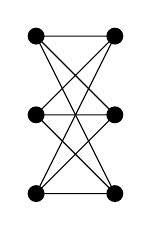
\begin{tikzpicture}
    \filldraw[fill=black, draw=black] (0, 0) circle [radius=0.1];
    \filldraw[fill=black, draw=black] (0, 1) circle [radius=0.1];
    \filldraw[fill=black, draw=black] (0, 2) circle [radius=0.1];
    \filldraw[fill=black, draw=black] (1, 0) circle [radius=0.1];
    \filldraw[fill=black, draw=black] (1, 1) circle [radius=0.1];
    \filldraw[fill=black, draw=black] (1, 2) circle [radius=0.1];
    \draw (1, 1) -- (0, 0) -- (1, 0) -- (0, 1) -- (1, 1) -- (0, 2) -- (1, 2) -- (0, 1);
    \draw (0, 0) -- (1, 2);
    \draw (0, 2) -- (1, 0);
  \end{tikzpicture} \\
  Now we begin the assigned examples:
  \begin{enumerate}
  \item
    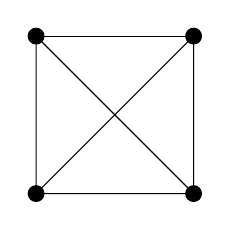
\begin{tikzpicture}
      \filldraw[fill=black, draw=black] (0, 0) circle [radius=0.1];
      \filldraw[fill=black, draw=black] (0, 2) circle [radius=0.1];
      \filldraw[fill=black, draw=black] (2, 0) circle [radius=0.1];
      \filldraw[fill=black, draw=black] (2, 2) circle [radius=0.1];
      \draw (0, 0) -- (2, 2) -- (2, 0) -- (0, 2) -- (0, 0) -- (2, 0);
      \draw (0, 2) -- (2, 2);
    \end{tikzpicture}
    \ \ and, for something that is planar:
    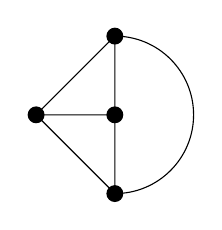
\begin{tikzpicture}
      \filldraw[fill=black, draw=black] (0, 1) circle [radius=0.1];
      \filldraw[fill=black, draw=black] (1, 0) circle [radius=0.1];
      \filldraw[fill=black, draw=black] (1, 1) circle [radius=0.1];
      \filldraw[fill=black, draw=black] (1, 2) circle [radius=0.1];
      \draw (1, 0) arc (-90:90:1cm);
      \draw (0, 1) -- (1, 1) -- (1, 2) -- (0, 1) -- (1, 0) -- (1, 1);
    \end{tikzpicture}
  \item
      A planar diagram of $K_{2, 3}$: \\
        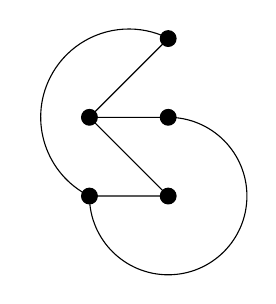
\begin{tikzpicture}
          \filldraw[fill=black, draw=black] (0, 0) circle [radius=0.1];
          \filldraw[fill=black, draw=black] (0, 1) circle [radius=0.1];
          \filldraw[fill=black, draw=black] (1, 0) circle [radius=0.1];
          \filldraw[fill=black, draw=black] (1, 1) circle [radius=0.1];
          \filldraw[fill=black, draw=black] (1, 2) circle [radius=0.1];
          \draw (1, 1) -- (0, 1) -- (1, 0) -- (0, 0);
          \draw (1, 2) -- (0, 1);
          \draw (0, 0) arc(-180:90:1cm);
          \draw (0, 0) arc(243.43:63.42:1.12cm);
        \end{tikzpicture}
  \end{enumerate}
\end{response}

\begin{theorem}[Jordan Curve Theorem, Do Not Prove] If $C$ is a continuous simple closed curve in a plane and two points $x$ and $y$ of $C$ are joined by a continuous simple arc $L$ such that $L \cap C = \{x, y\}$, then except for its endpoints $L$ is entirely contained in one of the two regions of $\R^2 \setminus C$.
\end{theorem}

\begin{exercise} Draw an example of the situation described in the Jordan Curve theorem which demonstrates that the conclusion of the Jordan Curve Theorem is not always obvious.
\end{exercise}

\begin{theorem}\leavevmode
\begin{enumerate}
    \item $K_{3,3}$ is not planar.
    \item $K_5$ is not planar.
\end{enumerate}
(Do not use Theorem \ref{thm:euler}).
\end{theorem}
\begin{proof}
\item Label the vertices of $K_{3,3}$ $m_1, m_2, m_3, n_1, n_2, n_3$ such that $m_i$ is adjacent to $n_j$ for any $i$ and $j$ and no other edges are present, as the definition of $K_{3,3}$ allows. Consider any arbitrary graph diagram $D$ of this graph. Define the \textit{trace} of a path $P$ of $G$ to be the curve that connects the arcs of $D$ that connect each given pair of vertices of the given path. We seek to prove that there exists a trace of some path $P$ that is not simple, for any arbitrary $D$. \\
  Let $C$ be the closed curve traced by the path $(n_1, m_1, n_2, m_2, n_1)$. If this curve is not simple, then $D$ is not planar. If it is simple, consider the simple continuous arc $L$ that is the trace of the path $(n_1, m_3, n_2)$. By the Jordan Curve Theorem, with the exception of the endpoints of $L$ the entire curve lies in one of the two regions $\mathbb{R}^2 \setminus C$. Call the open region of $\R^2 \setminus C$ the \textit{outside} of $C$, and call the other region the \textit{inside} of $C$. We have that, WLOG, $L$ lies inside of $C$: if it is not, simply switch $m_3$ and $m_2$. Now consider $n_3$. There are two cases: $n_3$ lies inside of $C$, or $n_3$ lies outside of $C$. (This is because the arc traced by $(m_1, n_3, m_2$ has to be entirely outside or inside of $C$ by the Jordan Curve Theorem. \\
  \textbf{Case 1: $n_3$ is inside of $C$.} \\
  Call $C_2$ the simple closed curve that is the trace of $(m_1, n_1, m_3, n_2, m_1)$. The region $C \setminus C_2$ lies outside of $C_2$ and is distinct from it except along the arc $L$ by the Jordan Curve Theorem. $n_3$ must lie in either $C \setminus C_2$ or $C_2$ if it lies in $C$ by definition. Regardless of which set it lies in, it lies in a different set to either $m_1$, which only lies in $C_2$, or $m_3$, which only lies in $C \setminus C_2$. WLOG assume that $n_3$ is in $C_2$ and thus lies in a different region to $m_3$. Consider the trace of $(m_1, n_3, m_2, n_1)$. This arc connects two points on $C_2$, but it has points both inside and outside of $C_2$. Therefore, by the contrapositive of the Jordan Curve Theorem, either $C_2$ is not simple (in which case $D$ is not planar) or this arc intersects $C_2$ at some point outside of its endpoints (in which case $D$ is also not planar). Thus, if $n_3$ is inside $C$, $D$ is not planar. \\
  \textbf{Case 2: $n_3$ is outside of $C$.} \\
  If $n_3$ lies on the outside of $C$, then the trace of $(m_1, n_1, m_3, n_2, m_2)$ is a simple continuous arc that is not entirely contained in either region of $C$: $n_3$ is outside $C$, but $m_3$ is inside $C$. Thus, by the contrapositive of the Jordan Curve Theorem, either $C$ is not simple and closed (in which case $D$ is not planar) or this arc intersects $C$ at a point besides its endpoints, in which case $D$ is not planar. Thus, if $n_3$ is outside $C$, $D$ is not planar.\\
  In all cases $D$ is not planar. This holds for any arbitrary $D$. Thus, the graph $K_{3, 3}$ is nonplanar.
\end{proof}

\begin{theorem} Any subgraph of a planar graph is planar.
\end{theorem}

\begin{corollary} Any supergraph of a nonplanar graph is nonplanar.
\end{corollary}

\begin{definition} Let $G$ and $H$ be graphs.
\begin{enumerate}
    \item If $G$ may be obtained from $H$ by replacing an edge $(x, y)$ of $H$ with another vertex $v$, and a pair of edges $(x, v), (v, y)$, then $G$ is said to be obtained from $H$ via an \textbf{edge expansion}.
    \item If $G$ may be obtained from $H$ by a finite sequence of edge expansions, then $G$ is an \textbf{expansion} of $H$.
    \item If $G$ is obtained from $H$ by a finite sequence of expansions and passing to supergraphs, then $G$ is said to be an \textbf{expanded supergraph} of $H$.
\end{enumerate}
\end{definition}

\begin{theorem} Let $G$ and $H$ be graphs. If $G$ is an expanded supergraph of $H$, then $G$ is a supergraph of an expansion of $H$.
\end{theorem}

\begin{theorem} Every expanded supergraph of $K_{3,3}$ or $K_5$ is nonplanar.
\end{theorem}

\begin{theorem}[Kuratowski's Theorem, Do Not Prove] A graph $G$ is nonplanar if and only if $G$ is an expanded supergraph of $K_{3,3}$ or $K_5$.
\end{theorem}

\begin{example} Construct an example of a ``large'' graph which is indeed planar by Kuratowski's Theorem.
\end{example}

\subsection{Euler's Formula}
\begin{definition} Given a planar graph diagram $D$ of a graph $G$, a \textbf{face} of $D$ is the set of all points in $\R^2 \setminus D$ that may be joined by a continuous arc in $\R^2 \setminus D$.  The number of faces of $D$ is denoted as $f(D)$ (or just $f$ or $f(G)$ if $D$ is clear from context.)
\end{definition}

\begin{theorem} If $G$ is a planar graph with planar diagrams $D_1$ and $D_2$, then $f(D_1) = f(D_2)$.
\end{theorem}

\begin{definition} A graph diagram $D$ is \textbf{polygonal} if it is planar, connected, and has the propery that every edge of $D$ borders on two distinct faces.
\end{definition}

\begin{theorem}[Euler]\label{thm:euler} If $G$ is polygonal then $v-e+f = 2$.
\end{theorem}

\begin{corollary} If $G$ is planar and connected, then $v-e+f = 2$.
\end{corollary}

\begin{corollary} $K_5$ and $K_{3,3}$ are nonplanar.
\end{corollary}

\begin{theorem} If $G$ is planar then $G$ has a vertex of degree $\leq 5$
\end{theorem}

\begin{definition} Let $d\in \mathbb{N}$.  A graph is \textbf{regular of degree} $d$ if all its vertices have degree $d$.
\end{definition}

\begin{examples} Construct an example of a connected graph with $v$ vertices which is regular of degree $d$ for $v = 5, 6,$ and $7$ and $d=2, 3,$ and $4$, if possible.  If it isn't possible, explain why.
\end{examples}

\begin{definition} A graph is \textbf{platonic} if it is polygonal, regular, and all its faces are bounded by the same number of edges.
\end{definition}

\begin{examples}\leavevmode
\begin{enumerate}
    \item Construct an example of a platonic graph which is regular of degree $4$.
    \item Construct an example of a polygonal, regular graph which is not platonic.
\end{enumerate}
\end{examples}

\noindent We now aim to classify the platonic graphs.  In order to do so, we'll need the following lemmas.

\begin{lemma} If $G$ is regular of degree $d$ then $e=\frac{dv}{2}$.
\end{lemma}

\begin{lemma} If $G$ is platonic of degree $d$, and $n$ is the number of edges bounding each face, then $f = dv/n$.
\end{lemma}

\begin{theorem}[Euclid] Apart from $K_1$ and the cyclic graphs, there are 5 platonic graphs.
\end{theorem}

%%% Local Variables:
%%% mode: latex
%%% TeX-master: "graph_theory_and_combinatorics"
%%% End:
